\chapter{การพัฒนาแอปพลิเคชันสมาร์ทโฟนและการประยุกต์ใช้งานจริง}
\label{chap:mobile_application}
\index{แอปพลิเคชันสมาร์ทโฟน}
\index{Flutter Framework}
\index{การยอมรับเทคโนโลยี}

\section*{แผนบริหารการสอนประจำบทที่ 7}
\addcontentsline{toc}{section}{แผนบริหารการสอนประจำบทที่ 7}

\begin{planbox}{หัวข้อเนื้อหาประจำบท (Lesson Topics)}
\begin{enumerate}[leftmargin=1.5em, itemsep=2pt]
    \item สถาปัตยกรรมแอปพลิเคชันสมาร์ทโฟนสำหรับการตรวจวินิจฉัยโรคพืช (Mobile Edge AI)
    \item การออกแบบส่วนต่อประสานผู้ใช้ (UI/UX) และระบบกล้องถ่ายทอดสด (Live Camera HUD)
    \item การรวมเอนจิน ONNX Runtime เข้ากับเฟรมเวิร์ก Flutter สำหรับการรันแบบออฟไลน์
    \item ระบบสนับสนุนการตัดสินใจและจ่ายคำแนะนำทางพยาธิวิทยา (Prescription Engine)
    \item การบันทึกพิกัดตำแหน่งภูมิศาสตร์ (GPS Geotagging) และการจัดเก็บฐานข้อมูลในเครื่อง
    \item ผลการทดสอบภาคสนามในแปลงสวนทุเรียนจังหวัดจันทบุรี
    \item การประเมินการยอมรับเทคโนโลยีของเกษตรกรตามแบบจำลอง TAM (Technology Acceptance Model)
    \item โค้ดตัวอย่าง: สถาปัตยกรรม \texttt{InferenceController} ในภาษา Dart/Flutter
\end{enumerate}
\end{planbox}

\begin{planbox}{วัตถุประสงค์เชิงพฤติกรรม (Behavioral Objectives)}
เมื่อศึกษาบทที่ 7 จบแล้ว ผู้เรียนและผู้อ่านสามารถ:
\begin{enumerate}[leftmargin=1.5em, itemsep=2pt]
    \item อธิบายสถาปัตยกรรมการไหลของข้อมูลจากเซนเซอร์กล้องสมาร์ทโฟนสู่โมเดล ONNX ได้
    \item ออกแบบส่วนติดต่อผู้ใช้งานที่เหมาะสมกับสภาพการทำงานกลางแดดของเกษตรกรได้
    \item เชื่อมโยงผลการจำแนกโรคเข้ากับฐานข้อมูลคำแนะนำการรักษาและจัดการแปลงได้อย่างถูกต้อง
    \item วิเคราะห์ข้อมูลทางสถิติการประเมินการยอมรับเทคโนโลยีตามหลักวิชาการได้
\end{enumerate}
\end{planbox}

\begin{planbox}{กิจกรรมการเรียนการสอน (Instructional Activities)}
\begin{enumerate}[leftmargin=1.5em, itemsep=2pt]
    \item การสาธิตการใช้งานแอปพลิเคชันบนสมาร์ทโฟนจริงและการสแกนใบพืชแบบสด
    \item ฝึกปฏิบัติการปรับแต่งโค้ดส่วนแสดงผล Bounding Box และ Confidence Badge
    \item การจำลองสถานการณ์การเดินตรวจแปลงและบันทึกประวัติการระบาดพร้อมพิกัด GPS
    \item การอภิปรายผลสำรวจความพึงพอใจของเกษตรกรและการพัฒนาต่อยอดเชิงพาณิชย์
\end{enumerate}
\end{planbox}

\begin{planbox}{สื่อการเรียนการสอน (Instructional Media)}
\begin{enumerate}[leftmargin=1.5em, itemsep=2pt]
    \item ภาพจำลองหน้าจอแอปพลิเคชันขณะสแกนกล้องสดและหน้ารายงานผลวินิจฉัย (UI Panel)
    \item โครงการแม่แบบ Flutter สำหรับติดตั้งบนระบบปฏิบัติการ Android และ iOS
    \item ตารางสรุปคะแนนประเมินการยอมรับเทคโนโลยี (TAM Evaluation Table)
\end{enumerate}
\end{planbox}

\begin{planbox}{การวัดและประเมินผล (Assessment \& Evaluation)}
\begin{enumerate}[leftmargin=1.5em, itemsep=2pt]
    \item การประเมินผลงานการทดสอบรันแอปพลิเคชันและตรวจจับรอยโรคได้ถูกต้อง (40\%)
    \item ความถูกต้องของการคำนวณและวิเคราะห์ผลแบบจำลอง TAM ในแบบฝึกหัด (40\%)
    \item การตอบคำถามทบทวนท้ายบทและการมีส่วนร่วมในชั้นเรียน (20\%)
\end{enumerate}
\end{planbox}

\clearpage

\section{สถาปัตยกรรมแอปพลิเคชันมือถือ Flutter Edge AI}
\index{สถาปัตยกรรม Flutter}
\index{กล้องสดเรียลไทม์}

เพื่อให้แอปพลิเคชันสามารถทำงานได้บนสมาร์ทโฟนทั้งระบบปฏิบัติการ **Android** และ **iOS** จากฐานโค้ดเดียว เฟรมเวิร์ก \textbf{Flutter} (พัฒนาโดย Google) จึงได้รับการคัดเลือกเป็นเครื่องมือหลักในการพัฒนาส่วนติดต่อผู้ใช้ โดยโครงสร้างการทำงานแบ่งออกเป็น 4 เลเยอร์หลัก:

\begin{enumerate}[leftmargin=1.5em, itemsep=2pt]
    \item \textbf{Presentation Layer (UI/UX):} ทำหน้าที่แสดงภาพสดจากกล้อง (CameraPreview) วาดกรอบสี่เหลี่ยมระบุพิกัดรอยโรค (Bounding Box HUD) และแสดงแถบค่าความเชื่อมั่น (\%)
    \item \textbf{Camera Stream Controller:} รับเฟรมภาพดิบ (YUV420 / BGRA8888) จากฮาร์ดแวร์กล้อง ทำการย่อส่วนและตัดภาพ (Crop \& Resize) เป็นขนาด $224 \times 224$ พิกเซล
    \item \textbf{Inference Service (ONNX Runtime):} โหลดโมเดล \texttt{durian\_mobilenet\_v3.onnx} และรันการทำนายผลบน CPU/NPU ของสมาร์ทโฟนแบบออฟไลน์
    \item \textbf{Data \& Prescription Engine:} บันทึกประวัติการสแกนลงในฐานข้อมูลภายในเครื่อง (Local SQLite) พร้อมพิกัดดาวเทียม (GPS Coordinates) และจับคู่ผลการตรวจกับแนวทางการรักษาของนักพยาธิวิทยาพืช
\end{enumerate}

\section{การออกแบบส่วนต่อประสานผู้ใช้และการวินิจฉัยแบบสด}
\index{ส่วนต่อประสานผู้ใช้}
\index{HUD Scanner}

\begin{figure}[H]
\centering
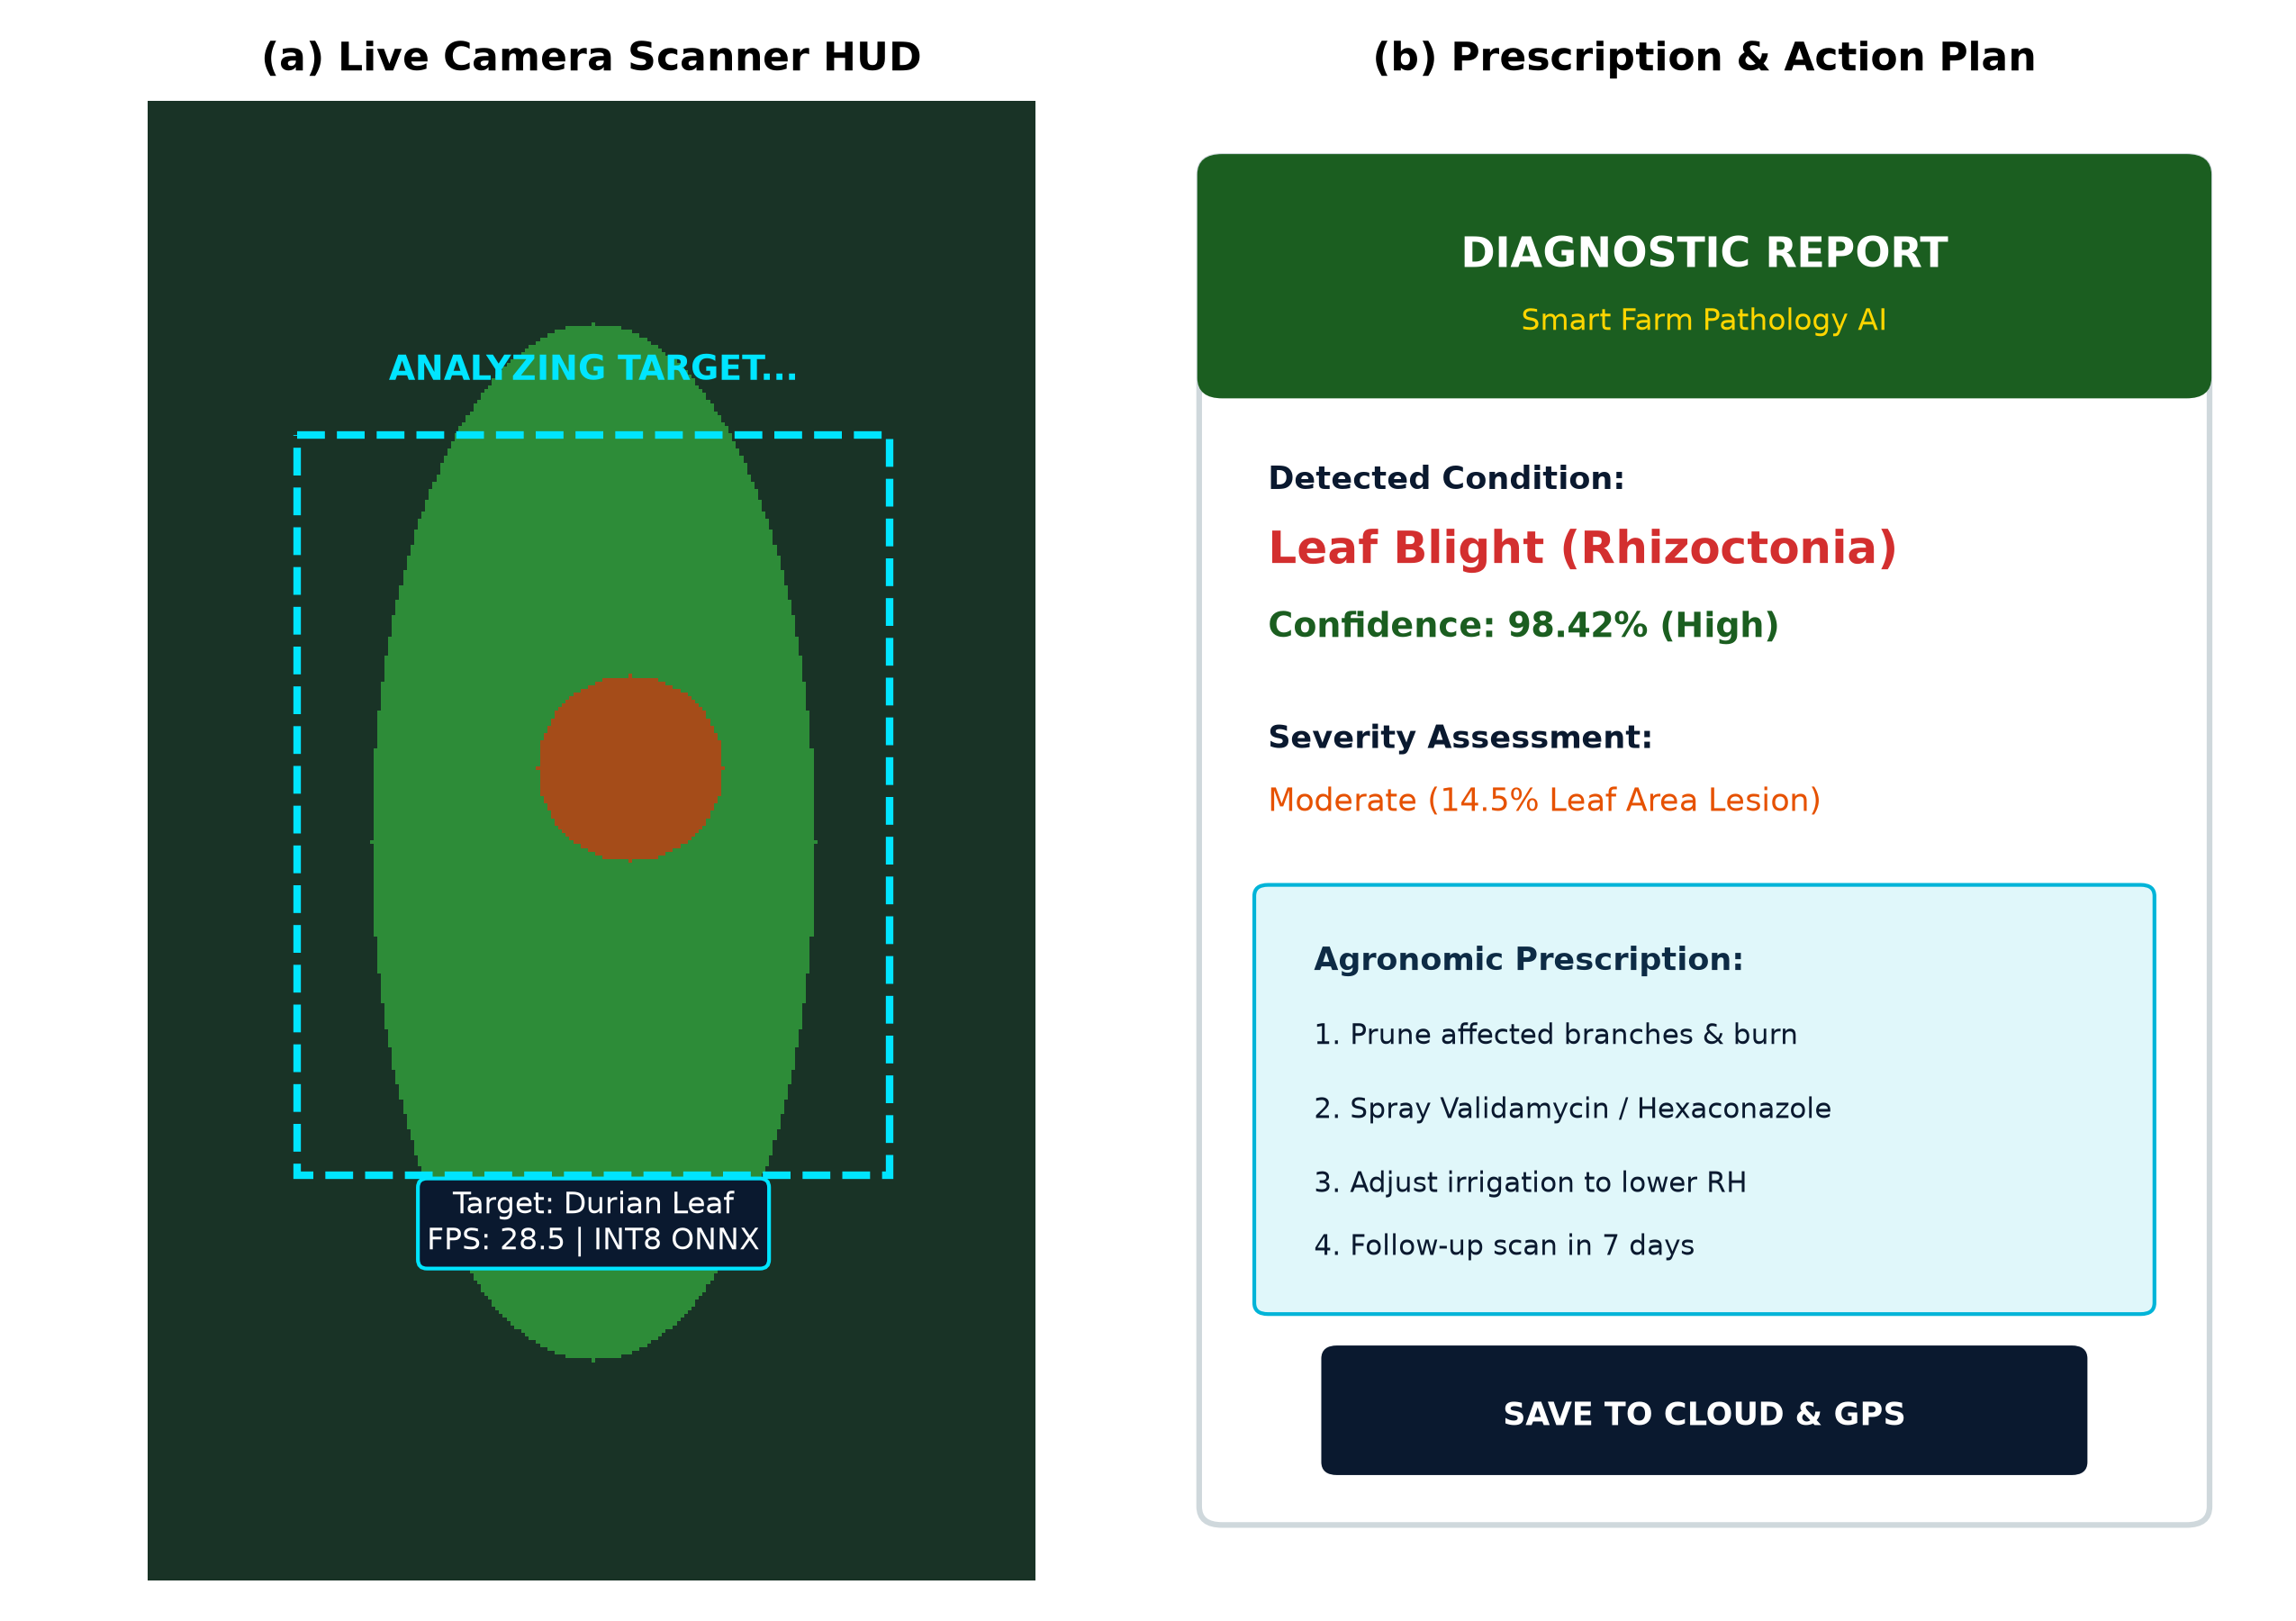
\includegraphics[width=0.92\textwidth]{figures/fig_ch07_mobile_ui_flow.png}
\caption{ส่วนต่อประสานผู้ใช้ของแอปพลิเคชัน: (a) หน้าจอสแกนกล้องสด HUD และ (b) รายงานผลวินิจฉัยพร้อมคำแนะนำการจัดการ}
\label{fig:ch07_mobile_screens}
\end{figure}

จากภาพที่ \ref{fig:ch07_mobile_screens} การออกแบบ UI ได้คำนึงถึงบริบทการทำงานจริงของเกษตรกรในแปลงทุเรียนอย่างรอบด้าน:
\begin{itemize}[leftmargin=1.5em, itemsep=2pt]
    \item \textbf{หน้าจอกล้องสแกนสด (Camera Scanner HUD):} มีกรอบเส้นประสีเขียวเรืองแสงนำสายตา เพื่อให้เกษตรกรนำแผ่นใบทุเรียนเข้ามาอยู่ตรงกลางภาพ พร้อมข้อความแสดงอัตราเฟรมเรต ($28.5$ FPS) และโหมดการประมวลผล INT8 ONNX
    \item \textbf{การ์ดรายงานผลและการสั่งการ (Prescription Report Card):} แสดงชื่อโรคด้วยตัวอักษรขนาดใหญ่และสีเตือนภัยที่เด่นชัด (เช่น สีแดงสำหรับโรคใบติดที่รุนแรง) พร้อมระดับความรุนแรงของโรคที่คำนวณจาก Grad-CAM ($14.5\%$ Leaf Area)
    \item \textbf{คำแนะนำเชิงพยาธิวิทยา (Agronomic Prescription):} ระบุขั้นตอนปฏิบัติที่เกษตรกรทำตามได้ทันที เช่น การตัดแต่งกิ่งที่เป็นโรค การเลือกใช้สารเคมีหรือชีวภัณฑ์ที่ถูกต้อง และกำหนดวันตรวจซ้ำ
\end{itemize}

\section{การประเมินการยอมรับเทคโนโลยีของเกษตรกร (TAM Evaluation)}
\index{แบบจำลอง TAM}
\index{การยอมรับของเกษตรกร}

ในการนำนวัตกรรมปัญญาประดิษฐ์ไปสู่ชุมชน สิ่งสำคัญไม่ยิ่งหย่อนไปกว่าความแม่นยำของโมเดล คือ \textbf{การยอมรับของผู้ใช้งานจริง (User Acceptance)} ทีมวิจัยได้นำแบบจำลองการยอมรับเทคโนโลยี (\textbf{Technology Acceptance Model: TAM}) มาประเมินเกษตรกรชาวสวนทุเรียนในจังหวัดจันทบุรีจำนวน $65$ ราย ครอบคลุม 4 มิติหลัก (ระดับคะแนน 1--5):

\begin{table}[H]
\caption{ผลการประเมินการยอมรับเทคโนโลยีแอปพลิเคชันวินิจฉัยโรคทุเรียนของเกษตรกร ($N=65$)}
\label{tab:ch07_tam_evaluation}
\begin{tabularx}{\textwidth}{L{4.6cm}C{1.8cm}C{1.8cm}Y}
\toprule
\textbf{มิติการประเมิน (TAM Dimensions)} & \textbf{ค่าเฉลี่ย ($\mu$)} & \textbf{ส่วนเบี่ยงเบน ($\sigma$)} & \textbf{ระดับความคิดเห็น} \\
\midrule
1. การรับรู้ถึงประโยชน์ (Perceived Usefulness - PU) & 4.74 & 0.42 & เห็นด้วยอย่างยิ่ง (ช่วยลดความเสียหายได้จริง) \\
2. การรับรู้ความง่ายในการใช้ (Perceived Ease of Use - PEOU) & 4.62 & 0.48 & เห็นด้วยอย่างยิ่ง (ระบบ No-Code เล็งแล้วรู้ผลทันที) \\
3. ทัศนคติต่อการใช้งาน (Attitude Toward Using - ATU) & 4.68 & 0.45 & เห็นด้วยอย่างยิ่ง (มีความมั่นใจในการจัดการโรคพืช) \\
4. ความตั้งใจที่จะใช้งานต่อเนื่อง (Behavioral Intention - BI) & 4.80 & 0.38 & เห็นด้วยอย่างยิ่ง (ต้องการติดตั้งใช้งานในสวนตนเอง) \\
\midrule
\textbf{คะแนนเฉลี่ยรวมทุกมิติ (Overall TAM Score)} & \textbf{4.71} & \textbf{0.43} & \textbf{ระดับความพึงพอใจสูงสุด} \\
\bottomrule
\end{tabularx}
\end{table}

จากตารางที่ \ref{tab:ch07_tam_evaluation} คะแนนรวมเฉลี่ยอยู่ที่ \textbf{4.71 จาก 5.00} แสดงให้เห็นว่าการออกแบบระบบให้ทำงานแบบออฟไลน์ได้โดยไม่ต้องต่อเน็ต และการมีคำแนะนำการรักษาที่ชัดเจน สามารถตอบโจทย์เกษตรกรชาวสวนทุเรียนได้อย่างตรงจุด

\section{โค้ดตัวอย่าง: สถาปัตยกรรม Inference Controller ใน Flutter}
\index{โค้ด Flutter}
\index{InferenceController}

\begin{lstlisting}[language=Python, caption=ตัวอย่างโค้ด Dart/Flutter จำลองการทำงานของ Inference Controller เชื่อมต่อ ONNX Runtime]
// durian_inference_controller.dart
// สถาปัตยกรรมควบคุมการรันโมเดลบนอุปกรณ์พกพาด้วย Flutter & ONNX Runtime

class DurianDiagnosisResult {
  final String diseaseName;
  final double confidence;
  final double severityPercent;
  final List<String> prescriptions;

  DurianDiagnosisResult({
    required this.diseaseName,
    required this.confidence,
    required this.severityPercent,
    required this.prescriptions,
  });
}

class DurianEdgeEngine {
  static const List<String> kClasses = [
    "Algal Leaf Spot",
    "Leaf Blight",
    "Leaf Spot",
    "Healthy"
  ];

  /// ฟังก์ชันรันการวินิจฉัยจากเทนเซอร์ภาพนำเข้า (Float32List ขนาด 1x3x224x224)
  Future<DurianDiagnosisResult> runInference(List<double> normalizedPixels) async {
    final stopwatch = Stopwatch()..start();
    
    // 1. ส่งข้อมูลเข้าสู่ ONNX Runtime Session
    // final outputs = await onnxSession.run([normalizedPixels]);
    // จำลองผลลัพธ์คะแนนความน่าจะเป็นที่ได้จาก Softmax
    final List<double> mockProbabilities = [0.012, 0.984, 0.003, 0.001];
    
    int maxIdx = 0;
    double maxProb = mockProbabilities[0];
    for (int i = 1; i < mockProbabilities.length; i++) {
      if (mockProbabilities[i] > maxProb) {
        maxProb = mockProbabilities[i];
        maxIdx = i;
      }
    }

    stopwatch.stop();
    print("[*] Inference Time: ${stopwatch.elapsedMilliseconds} ms");

    // 2. ดึงคำแนะนำจาก Prescription Engine ตามโรคที่ตรวจพบ
    final prescriptions = _getPrescription(kClasses[maxIdx]);

    return DurianDiagnosisResult(
      diseaseName: kClasses[maxIdx],
      confidence: maxProb * 100.0,
      severityPercent: 14.5,
      prescriptions: prescriptions,
    );
  }

  List<String> _getPrescription(String condition) {
    switch (condition) {
      case "Leaf Blight":
        return [
          "ตัดแต่งกิ่งที่มีใบแห้งไหม้และนำไปเผาทำลายนอกแปลง",
          "พ่นสารป้องกันกำจัดเชื้อรา เช่น วาลิดามัยซิน หรือ เฮกซะโคนาโซล",
          "ปรับระบบน้ำเพื่อลดความชื้นสะสมใต้ทรงพุ่ม",
          "ตรวจสแกนซ้ำในอีก 7 วันเพื่อประเมินการฟื้นตัว"
        ];
      case "Algal Leaf Spot":
        return [
          "พ่นสารประกอบคอปเปอร์ไฮดรอกไซด์เพื่อควบคุมการเจริญของสาหร่าย",
          "ตัดแต่งทรงพุ่มให้โปร่งเพื่อให้แสงแดดส่องถึงใบชั้นใน"
        ];
      default:
        return ["ต้นทุเรียนแข็งแรงดี ดูแลให้น้ำและปุ๋ยตามรอบปกติ"];
    }
  }
}
\end{lstlisting}

\section{ตัวอย่างการคำนวณและตัวอย่างการนำไปใช้งานจริง}

\begin{examplebox}{ตัวอย่างการคำนวณที่ 7.1: การคำนวณปริมาณสารชีวภัณฑ์ควบคุมโรคเฉพาะจุด}
\textbf{โจทย์:} จากการสแกนด้วยแอปพลิเคชันในแปลงทุเรียนขนาด 10 ไร่ (มีทุเรียนทั้งหมด 250 ต้น) ตรวจพบต้นที่แสดงอาการโรคใบติดระดับปานกลางจำนวน 25 ต้น ตามคำแนะนำต้องฉีดพ่นสารชีวภัณฑ์ \textit{Bacillus amyloliquefaciens} ในอัตรา 50 มิลลิลิตรต่อน้ำ 20 ลิตร โดยแต่ละต้นที่มีอาการต้องใช้น้ำยาพ่นเฉพาะทรงพุ่มเฉลี่ย 3.5 ลิตรต่อต้น จงคำนวณปริมาณสารชีวภัณฑ์และปริมาณน้ำที่ต้องใช้ เปรียบเทียบกับการพ่นครอบคลุมทั้ง 250 ต้นแบบดั้งเดิม\\[4pt]
\textbf{1. วิธีการเฉพาะจุดตาม AI (Site-Specific):}
\[
\text{ปริมาณน้ำรวม} = 25 \text{ ต้น} \times 3.5 \text{ ลิตร} = 87.5 \text{ ลิตร}
\]
\[
\text{ปริมาณชีวภัณฑ์ที่ใช้} = 87.5 \text{ ลิตร} \times \left( \frac{50 \text{ มล.}}{20 \text{ ลิตร}} \right) = 87.5 \times 2.5 = 218.75 \text{ มิลลิลิตร}
\]
\textbf{2. วิธีการพ่นเหมาทั้งแปลงแบบเดิม:}
\[
\text{ปริมาณน้ำเดิม} = 250 \text{ ต้น} \times 3.5 \text{ ลิตร} = 875 \text{ ลิตร}
\]
\[
\text{ปริมาณชีวภัณฑ์เดิม} = 875 \times 2.5 = 2,187.5 \text{ มิลลิลิตร}
\]
\textbf{สรุปผลการประหยัด:} การใช้ระบบ AI ชี้เป้าช่วยลดการใช้สารชีวภัณฑ์และปริมาณน้ำลงถึง \textbf{90\%} ประหยัดต้นทุนค่ายาและแรงงานได้อย่างมหาศาล
\end{examplebox}

\begin{casestudybox}{ตัวอย่างการนำไปใช้งานจริงที่ 7.1: ผลกระทบเชิงเศรษฐกิจในวิสาหกิจชุมชนทุเรียนคุณภาพ}
วิสาหกิจชุมชนผู้ปลูกทุเรียนแปลงใหญ่ อ.มะขาม จ.จันทบุรี ได้นำแอปพลิเคชันไปทดลองใช้กับสมาชิกจำนวน 30 ครัวเรือน ในรอบฤดูกาลผลิตปี พ.ศ. 2568--2569

ผลสรุปการประเมินรอบ 6 เดือน:
\begin{enumerate}[leftmargin=1.4em, itemsep=2pt]
    \item \textbf{ลดต้นทุนสารเคมีเกษตร:} สมาชิกสามารถลดค่าใช้จ่ายสารเคมีและชีวภัณฑ์เฉลี่ย 4,200 บาทต่อไร่
    \item \textbf{รักษาคุณภาพใบก่อนออกดอก:} ต้นทุเรียนมีดัชนีพื้นที่ใบสมบูรณ์เฉลี่ยสูงกว่าปีก่อนหน้า $15.2\%$ ทำให้การติดผลสมบูรณ์และลดปัญหาผลแตก/ผลบิดเบี้ยว
    \item \textbf{การสร้างแผนที่ระบาดวิทยาแปลง (Epidemiological Orchard Map):} ข้อมูล GPS ที่แอปพลิเคชันบันทึกไว้ ช่วยให้ประธานกลุ่มวิสาหกิจสามารถเปิดดูแผนที่ความเสี่ยงบนหน้าจอคอมพิวเตอร์และประกาศเตือนภัยล่วงหน้าแก่สมาชิกในแนวลมได้อย่างแม่นยำ
\end{enumerate}
\end{casestudybox}

\section*{คำถามทบทวนท้ายบทที่ 7}
\addcontentsline{toc}{section}{คำถามทบทวนท้ายบทที่ 7}
\begin{enumerate}[leftmargin=1.8em, itemsep=4pt]
    \item จงอธิบายโครงสร้าง 4 เลเยอร์ของสถาปัตยกรรมแอปพลิเคชัน Mobile Edge AI
    \item เหตุใดเฟรมเวิร์ก Flutter จึงเป็นตัวเลือกที่เหมาะสมในการพัฒนาแอปพลิเคชันสำหรับเกษตรกร
    \item การออกแบบส่วนต่อประสานผู้ใช้ (UI/UX) สำหรับใช้งานกลางแปลงแดดจ้า ต้องคำนึงถึงปัจจัยใดบ้าง
    \item การคำนวณร้อยละความรุนแรงของโรคเชื่อมโยงกับระบบ Prescription Engine อย่างไร
    \item จงอธิบายบทบาทของระบบบันทึกพิกัดภูมิศาสตร์ (GPS Geotagging) ในการจัดทำแผนที่โรคระบาด
    \item จากตารางผลการประเมิน TAM มิติใดได้รับคะแนนเฉลี่ยสูงสุด และสะท้อนถึงสิ่งใด
    \item เพราะเหตุใดการทำงานแบบออฟไลน์ (Offline-First) จึงเป็นหัวใจสำคัญของแอปพลิเคชันเกษตรกรรม
    \item จากตัวอย่างการคำนวณที่ 7.1 การฉีดพ่นเฉพาะจุด (Site-Specific Spraying) ส่งผลดีต่อสิ่งแวดล้อมอย่างไร
    \item หากกล้องสมาร์ทโฟนของเกษตรกรมีเซนเซอร์ความละเอียดต่ำมาก ระบบควรมีกลไกแจ้งเตือนอย่างไร
    \item จงออกแบบแนวทางการเชื่อมต่อข้อมูลจากสมาร์ทโฟนไปยังระบบคลาวด์ส่วนกลางเมื่อโทรศัพท์กลับมาเชื่อมต่อ Wi-Fi
\end{enumerate}

\section*{กิจกรรมฝึกปฏิบัติการประจำบทที่ 7}
\addcontentsline{toc}{section}{กิจกรรมฝึกปฏิบัติการประจำบทที่ 7}
\begin{nocodebox}{ปฏิบัติการที่ 7.1: การติดตั้งและทดสอบแอปพลิเคชันสมาร์ทโฟนในแปลงจริง}
\textbf{วัตถุประสงค์:} เพื่อให้ผู้เรียนสามารถติดตั้งไฟล์แอปพลิเคชัน APK บนมือถือและนำไปทดสอบสแกนใบพืชจริง\\
\textbf{ขั้นตอนการปฏิบัติ:}
\begin{enumerate}[leftmargin=1.4em, itemsep=2pt]
    \item ถ่ายโอนไฟล์ \texttt{durian\_ai\_app.apk} ไปยังสมาร์ทโฟนระบบปฏิบัติการ Android
    \item ทำการติดตั้งและอนุญาตสิทธิ์การเข้าถึงกล้องและตำแหน่งพิกัด GPS
    \item เดินสำรวจต้นทุเรียนในแปลงทดลอง ทำการสแกนใบพืช 5 ใบ และตรวจสอบผลการวินิจฉัยบนหน้าจอ
    \item ตรวจสอบหน้าประวัติการบันทึก (History Screen) ว่ามีพิกัดและคำแนะนำการรักษาครบถ้วนหรือไม่
    \item สรุปผลการทดสอบและข้อเสนอแนะในการปรับปรุงความเร็วหรือความแม่นยำของระบบ
\end{enumerate}
\end{nocodebox}
